%%%%%%%%%%%%%%%%%%%%%%%%%%%%%%%%%%%%%%%%%%%%%%%%%%%%%%%%%%%%
%%% ELIFE ARTICLE TEMPLATE
%%%%%%%%%%%%%%%%%%%%%%%%%%%%%%%%%%%%%%%%%%%%%%%%%%%%%%%%%%%%
%%% PREAMBLE 
\documentclass[9pt,lineno]{elife}
% Use the onehalfspacing option for 1.5 line spacing
% Use the doublespacing option for 2.0 line spacing
% Please note that these options may affect formatting.
% Additionally, the use of the \newcommand function should be limited.

\usepackage{lipsum} % Required to insert dummy text
\usepackage[version=4]{mhchem}
\usepackage{siunitx}
\DeclareSIUnit\Molar{M}

%%%%%%%%%%%%%%%%%%%%%%%%%%%%%%%%%%%%%%%%%%%%%%%%%%%%%%%%%%%%
%%% ARTICLE SETUP
%%%%%%%%%%%%%%%%%%%%%%%%%%%%%%%%%%%%%%%%%%%%%%%%%%%%%%%%%%%%
\title{Robust method for measuring aminoacylation through tRNA-seq}

\author[1,2]{Kristian Davidsen}
\author[1*]{Lucas B Sullivan}
\affil[1]{Fred Hutchinson Cancer Center}
\affil[2]{Molecular and cellular biology program, University of Washington}

\corr{sullivan@fredhutch.org}{LBS}

%%%%%%%%%%%%%%%%%%%%%%%%%%%%%%%%%%%%%%%%%%%%%%%%%%%%%%%%%%%%
%%% ARTICLE START
%%%%%%%%%%%%%%%%%%%%%%%%%%%%%%%%%%%%%%%%%%%%%%%%%%%%%%%%%%%%

\begin{document}

\maketitle

\begin{abstract}
Please provide an abstract of no more than 150 words. Your abstract should explain the main contributions of your article, and should not contain any material that is not included in the main text.

Furthermore, we provide code with boilerplate example (\url{https://github.com/krdav/tRNA-charge-seq}) \\ \ \\
\end{abstract}


\section{Introduction}
Quantification of transfer RNA (tRNA) aminoacylation levels has been performed using radiolabeling \citep{Wolfson2002-gp}, Northern blotting \citep{Ho1987-ug, Varshney1991-zp, Stenum2017-wn}, DNA microarrays \citep{Dittmar2005-va} and high-throughput sequencing \citep{Evans2017-st}.
While the radiolabeling approach is very accurate, it is limited to purified tRNAs undergoing lab manipulation.
Northern blotting uses differential migration of acylated tRNA during electrophoresis to measure acylation levels.
However, this has many known limitations such as cross-binding probes, low sensitivity, low throughput when testing multiple tRNAs, small or no separation between aminoacylated and unaminoacylated tRNA etc.
Chemical differentiation of acylated tRNAs combined with DNA microarrays were introduced to circumvent the problems with Northern blotting but were superseded by high-throughput sequencing enabling quantification on all tRNAs in one experiment.

Chemical differentiation of acylated tRNAs was achieved by using the Malaprade reaction to attack the 2,3-dihydroxyls on the 3' ribose of unaminoacylated tRNA, causing ring opening and destabilization.
The destabilized base is then specifically eliminated using high pH and heat.
Aminoacylated tRNAs are protected from the Malaprade reaction due to esterification of one of the 3' ribose hydroxyls.
The chain of reactions was characterized and used extensively in the past in an effort to sequence RNA molecules \citep{Whitfeld1953-ca, Whitfeld1954-wl, Khym1961-xf, Neu1964-hu}, and while futile for RNA sequencing, it has proven a highly useful method to "tag" unaminoacylated tRNAs by introducing a single base truncation.
We shall refer to this chain of reactions as the "Whitfeld reaction".

The accuracy and robustness of the aminoacylation measurement depends on two parts: the completeness of the Whitfeld reaction and the quality of tRNA sequencing.
A major problem in tRNA sequencing is base modifications known to be numerous on tRNAs.
These can lead to stalling, wrong base incorporation, skipping or falloff during the reverse transcription step of the sequencing protocol \citep{Motorin2007-nb}.
Reverse transcriptase is most severely affected by base modifications disrupting the Watson–Crick base pairing, while other modifications are often less affected or silent \citep{Wang2021-fc}.
To increase readthrough the demethylase AlkB has been used \citep{Zheng2015-kj}, while more recently optimization of incubation conditions, including low salt and extended incubation time, has shown large increases in readthrough \citep{Behrens2021-gb}.
But other factors can lead to errors in tRNA sequencing such as low RNA integrity, incomplete deacylation prior to adapter ligation, adapter ligation bias, PCR amplification bias and problems in read alignment.

Adapter ligation bias is a well documented problem in small RNA sequencing \citep{Fuchs2015-nb, Zhuang2012-nu} receiving little attention in most tRNA sequencing protocols where it is particularly problematic because adapters often incorporate a barcode for sample multiplexing.
The problem is further exacerbated when tRNA sequencing is coupled with the Whitfeld reaction because this creates different sequence contexts for aminoacylated and unaminoacylated tRNAs.
The best solution to ligation bias is to optimize conditions such that the ligation goes to completion.
The 3' end of the cloverleaf tRNA structure contains four nucleotides not participating in the basepairing of the acceptor stem: the discriminator base followed by the invariant CCA-end.
These free nucleotides can be engaged in basepairing by an oligo splint designed to guide the ligation of the adapter and this approach has shown high tRNA specificity and ligation efficiency \cite{Shigematsu2017-tv, Smith2015-ht}.

new block, something

Read mapping is another known problem for tRNA sequencing.
It arises due to the high error-rate of the reverse transcriptase reading through modified bases resulting in frequent base misincorporations or skipping.
Combined with the short nature of tRNAs, reads will frequently not have any region with a continuous stretch of more then 15 nt. that perfectly match its reference.
This is a problem for almost all alignment algorithms because they rely on some variation of subsequence matching for heuristics to enable speed-up.
The problem has been addressed by clustering of the reference sequences \citep{Hoffmann2018-uz} as well as masking known modified positions in the reference sequences \citep{Behrens2021-gb}.

In recent years many variations of the tRNA sequencing methods have been published \citep{Wang2021-fc, Zheng2015-kj, Shigematsu2017-tv, Erber2020-qg, Thomas2021-fi, Lucas2023-vm, Pinkard2020-yd, Warren2021-wt, Yamagami2022-yb} but only few couple it with the Whitfeld reaction to probe aminoacylation levels \citep{Evans2017-st, Behrens2021-gb, Watkins2022-er} and even less is known about the accuracy of these measurements.
Here, we present an up-to-date method that ingrates the best developments from tRNA sequencing with an improved version of the Whitfeld reaction to accurately measure tRNA aminoacylation.
We perform validations of the quantitative capabilities of the method and analyse the different possible modes of failure.
Finally, we provide a code repository to enable further improvement of read mapping using non-heuristic alignment (\url{https://github.com/krdav/tRNA-charge-seq}).



\section{Results}


After oxidation yielding a dialdehyde, the terminal base removal in the Whitfeld reaction is catalyzed by a combination of high temperature and pH.
In the work by Whitfeld \citep{Whitfeld1954-wl} glycine was used, later lysine and other primary amines were used \citep{Khym1961-xf} as well as boric acid \citep{randerath1973sequence}.
It has been proposed that in the amine catalyzed cleavage the phosphoric ester linkage is broken by a $\beta$-elimination reaction \citep{Rammler1971-mt, uziel1973periodate} yielding an unsaturated product [see figure; Whitfeld reaction], but the reaction is complex, involving several semi-stable intermediates and different pathways depending on the pH \citep{Uziel1975-ja}.








\subsection{Level 2 Heading}

\lipsum[3]

\subsubsection{Level 3 Heading}

\lipsum[5]

\paragraph{Level 4 Heading}
\lipsum[7]


And look here is a duck \FIG{fig1}.






\begin{figure}[ht!]
\centering
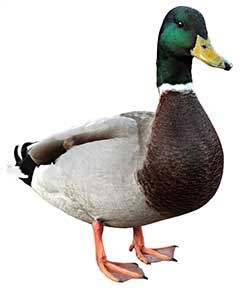
\includegraphics[height=2cm]{figures/duck.jpg}
\caption{
First figure: method summary, oligo design (maybe just illustrations)
}
\label{fig:fig1}
\end{figure}


\begin{figure}[ht!]
\centering
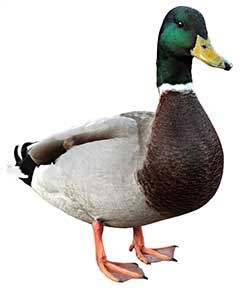
\includegraphics[height=2cm]{figures/duck.jpg}
\caption{
Second figure: method optimization, improved Whitfeld reaction, ligation completion etc. (mostly gel images)
}
\label{fig:fig2}
\end{figure}

\figsupp[Shorter caption for main text.]
{This is a supplementary figure's full caption, which will be used at the end of the manuscript. 
  \figsuppdata{A data source; see \url{https://doi.org/xxx}}
  \figsuppdata{Another data source.}
  \figsuppsrccode{And the source code.}}
{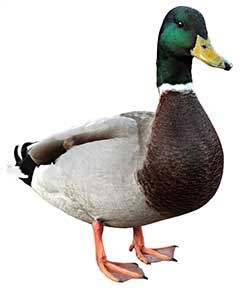
\includegraphics[width=6cm]{figures/duck.jpg}}\label{figsupp:sfig2_1}

\figsupp[Shorter caption for main text.]
{This is a supplementary figure's full caption, which will be used at the end of the manuscript. 
  \figsuppdata{A data source; see \url{https://doi.org/xxx}}
  \figsuppdata{Another data source.}
  \figsuppsrccode{And the source code.}}
{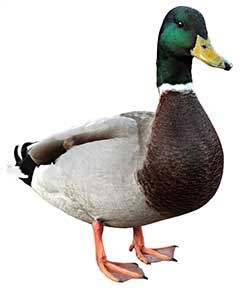
\includegraphics[width=6cm]{figures/duck.jpg}}\label{figsupp:sfig2_2}






\begin{figure}[ht!]
\centering
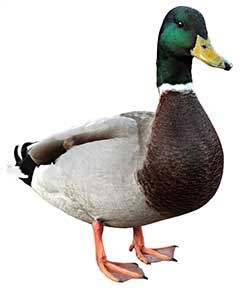
\includegraphics[height=2cm]{figures/duck.jpg}
\caption{
Third figure: alignment optimization, comparison to Behrens, coverage and mutation plots etc.
}
\label{fig:fig3}
\end{figure}





\begin{figure}[ht!]
\centering
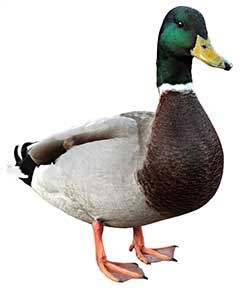
\includegraphics[height=2cm]{figures/duck.jpg}
\caption{
Fourth figure: replication with all barcode samples
}
\label{fig:fig4}
\end{figure}


\begin{figure}[ht!]
\centering
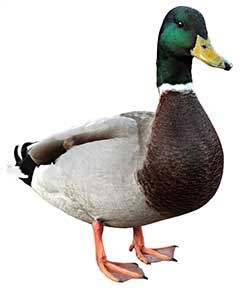
\includegraphics[height=2cm]{figures/duck.jpg}
\caption{
Fifth figure: charge titration validation
}
\label{fig:fig5}
\end{figure}


\begin{figure}[ht!]
\centering
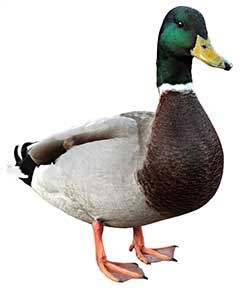
\includegraphics[height=2cm]{figures/duck.jpg}
\caption{
Sixth figure: charge half-life
}
\label{fig:fig6}
\end{figure}















\begin{table}[bt]
\caption{\label{tab:example}Automobile Land Speed Records (GR 5-10).}
% Use "S" column identifier to align on decimal point 
\begin{tabular}{S l l l r}
\toprule
{Speed (mph)} & Driver          & Car                        & Engine    & Date     \\
\midrule
407.447     & Craig Breedlove & Spirit of America          & GE J47    & 8/5/63   \\
413.199     & Tom Green       & Wingfoot Express           & WE J46    & 10/2/64  \\
434.22      & Art Arfons      & Green Monster              & GE J79    & 10/5/64  \\
468.719     & Craig Breedlove & Spirit of America          & GE J79    & 10/13/64 \\
526.277     & Craig Breedlove & Spirit of America          & GE J79    & 10/15/65 \\
536.712     & Art Arfons      & Green Monster              & GE J79    & 10/27/65 \\
555.127     & Craig Breedlove & Spirit of America, Sonic 1 & GE J79    & 11/2/65  \\
576.553     & Art Arfons      & Green Monster              & GE J79    & 11/7/65  \\
600.601     & Craig Breedlove & Spirit of America, Sonic 1 & GE J79    & 11/15/65 \\
622.407     & Gary Gabelich   & Blue Flame                 & Rocket    & 10/23/70 \\
633.468     & Richard Noble   & Thrust 2                   & RR RG 146 & 10/4/83  \\
763.035     & Andy Green      & Thrust SSC                 & RR Spey   & 10/15/97\\
\bottomrule
\end{tabular}

\medskip 
Source: \url{https://www.sedl.org/afterschool/toolkits/science/pdf/ast_sci_data_tables_sample.pdf}

\tabledata{This is a description of a data source.}\label{tabdata:first}
\tablesrccode{This is a description of a source code.}\label{tabsrccode:first}

\end{table}

\subsection{Level 2 Heading}

\lipsum[3]

\subsubsection{Level 3 Heading}

\lipsum[5]

\paragraph{Level 4 Heading}
\lipsum[7]

\section{Discussion}

% For discussion secion:
% Future could be NanoPore sequencing; however, still considerable problems for measuring aminoacylation accurately:
% It all depends on the CCA vs CC i.e. here very high quality is necessary
% Thomas et al. 2021 showed the way forward on NanoPore tRNA sequencing but still major caveats
% Lucas et al. (2023 NanoPore paper) solved many of the problems but still only gets around 50\% read alignment despite long reads. We get X\%.
% Still not as high throughput
% However, and hopefully, if these barriers can be overcome direct sequencing offered by NanoPore would be preferable 

Histidine is not suitable for tRNAseq using splint ligation barcodes due to the additional G added to the 5' end and shielding the discriminator base from base pairing (Heinemann 2011)


Regarding alignment mention well developed software such as ShapeMapper 2 as an alternative, although ShapeMapper employs bowtie/STAR for read mapping.



Limitations:
Not rigorously tested with tRNA abundances in mind.



Future directions:
Plenty of room to further optimize the RT reaction.
New and old enzymes such as group II intron RT and non-LTR RT (Upton 2021) with some commercially available e.g. Induro Reverse Transcriptase.
Temperature and buffer composition.
Enhancers.


Investigate the effect of deacylation on tRNA abundance.











\section{Methods and Materials}


For ligation tests human tRNA was isolated from whole cell RNA from H1299 cells.
After deacylation at 45C in 1 M lysine (pH=8) for 4 hours, the tRNA fraction was isolated on a denaturing gel.

For testing 3'-end base cleavage, spike-in control and ligation tests two RNA oligos were acquired from IDT, both with the sequence of \textit{E. coli} tRNA$\text{Lys}$ and ending on either CC or CCA.
These were purified on a denaturing gel to minimize truncation products.

For spike-in control an RNA oligo was acquired from IDT with the sequence of \textit{E. coli} tRNA$\text{Thr}$ and ending on CCAA.
On this oligo the Whitfeld reaction was performed, omitting the dephosphorylation step and gel purifying the resulting product to generate tRNA$\text{Thr}$ and ending on CCA-Phos.
A sample of this was dephosphorylated using rSAP, purified and mixed in a one-to-one ratio with its phosphorylated parent.
This 50\% 3'-phosphorylated \textit{E. coli} tRNA$\text{Thr}$ is used as a spike-in to simulate a 50\% aminoacylated tRNA.




Four types of sequenced controls were used: non-oxidized tRNA, deacylated tRNA, \textit{E. coli} tRNA$\text{Lys}$ spike-in and 50\% 3'-phosphorylated \textit{E. coli} tRNA$\text{Thr}$ spike-in.
Samples of non-oxidized tRNA were prepared similarly to normal samples but with NaIO4 swapped to NaCl.
Samples of deacylated tRNA were prepared by first performing an initial deacylation step on the input RNA by incubation at 45C for 4 h in 1 M lysine (pH=8).
For all non-\textit{E. coli} samples, the above mentioned \textit{E. coli} tRNA$\text{Lys}$ oligo ending on CCA and 50\% 3'-phosphorylated \textit{E. coli} tRNA$\text{Thr}$ was spiked-in to each RNA samples before the NaIO4 oxidation step.


Ligation tests using pre-adenylated single stranded adapters.
Figure reference (probably Fig 2, S9).
[Describe design and adenylation of adapters.]
Ligations were performed using 40 ng tRNA, a ~5x excess of pre-adenylated adapters, 17.5\% PEG-8000, 200 U Rnl2tr KQ ligase (NEB) and the vendor provided buffer.





\subsection*{Oligo design}
Design building on experience from Ignolia, Behrens and YAMAT-seq papers.

Using splint directed ligation, one splint for CC ending and one for CCA ending.

Using SpC3 to block ligation of the splint to the tRNA.

RT-oligo: similar design as Ignolia and Behrens, with a 5' phosphorylated random A/G base to increase circular ligation efficiency.
We chose to add an additional 9 random bases following the random A/G base and refer to this as the unique molecular identifier (UMI).
This UMI has 524288 possible sequences and since the input RNA molecules are several orders of magnitude more abundant it is not strictly speaking a molecular identifier.
Nevertheless, it serves three purposes: 1) increase 5' sequence diversity for improved sequencing for read P1, 2) decrease any potential circular ligase primary sequence preference and 3) serve as a quality control for the library prep.
As a quality control, the number of observed UMI sequences is compared with the number expected ($E[X]$) given the number of random UMI draws ($n$) i.e. sequencing reads for the particular sample and the number of possible UMIs ($k$).
The number of expected UMI sequences is calculated as:
$$
E[X] = n \left[ 1 - \left(\frac{n-1}{n} \right)^k \right]
$$


Using varying adapter lengths to shift the sequencing "reading frame"  to avoid the 3' CCA sequence to cause near-zero sequence diversity on the read P2.

Illumina library oligos are designed as a Truseq dual index library with combined i5 and i7 indices.
Library oligos are synthesized with a phosphorothioate bond between the last two nucleotides to prevent degradation by KAPA HiFi Polymerase [Behrens].











Guidelines can be included for standard research article sections, such as this one. 

\lipsum[3]

\section{Some \LaTeX{} Examples}
\label{sec:examples}

Use \verb|\section| and \verb|\subsection| commands to organize your document. \LaTeX{} handles all the formatting automatically. Use \verb|\label| and \verb|\nameref| commands for cross-referencing sectional headings: the usual \verb|\ref| will not work, as this template uses unnumbered sectional headings.

\subsection{Figures and Tables}

Use the table and tabular commands for basic tables --- see \TABLE{example}, for example. 

You can upload a figure (JPEG, PNG or PDF) using the project menu. To include it in your document, use the \verb|\includegraphics| command as in the code for \FIG{view}. 

For a half-width figure or table with text wrapping around it, use 

\begin{verbatim}
\begin{wrapfigure}{l}{.46\textwidth}
  \includegraphics[width=\hsize]{...}
  \caption{...}\label{...}
\end{wrapfigure}
\end{verbatim}
%
as in \FIG{halfwidth}. For tables:

\begin{verbatim}
\begin{wraptable}{l}{.46\textwidth}{
  \begin{tabular}{...}
  ...
  \end{tabular}}
  \caption{...}\label{...}
\end{wraptable}
\end{verbatim}

Be careful with these, though, as they may behave strangely near page boundaries, sectional headings, or in the neighbourhood of lists or too many floats.

Labels for main videos can be added with \verb|\video| e.g.

\video{Ths is a description of a main video.\label{video:mv1}
  \videodata{This is a description of a video data source.}\label{viddata:first}
  \videodata{This is a description of another video data source.}\label{viddata:second}
  \videosrccode{This is a description of a video source code.}\label{vidsrccode:first}
}


Labels for video supplements can be added within \texttt{figure} environments, after the \texttt{caption}, using the \verb|\videosupp| command: see \VIDEOSUPP[view]{sv1} for an example.

If you use the following prefixes for your \verb|\label|:
%
\begin{description}
\item[Figures] \texttt{fig:}, e.g.~\verb|\label{fig:view}|
\item[Figure Supplements] \texttt{figsupp:}, e.g.~\verb|\label{figsupp:sf1}|\\
(we'll assume \texttt{figsupp:sf1} is a figure supplement of \texttt{fig:view} in our example)
\item[Figure source data] \texttt{figdata:}, e.g.~\verb|\label{figdata:first}|
\item[Figure source code] \texttt{figsrccode:},
\item[Videos] \texttt{video:}, e.g.~\verb|\label{video:mv1}|
\item[Video source data] \texttt{viddata:}, e.g.~\verb|\label{figdata:first}|
\item[Video source code] \texttt{vidsrccode:},
\item[Video supplements] \texttt{videosupp:}, e.g.~\verb|\label{videosupp:sv1}|
\item[Tables] \texttt{tab:}, e.g.~\verb|\label{tab:example}|
\item[Table source data] \texttt{tabdata:}, e.g.~\verb|\label{tabdata:first}|
\item[Table source code] \texttt{tabsrccode:},e.g.~\verb|\label{tabsrccode:first}|
\item[Equations] \texttt{eq:}, e.g.~\verb|\label{eq:CLT}|
\item[Boxes] \texttt{box:}, e.g.~\verb|\label{box:simple}|
\end{description}
%
you can then use the convenience commands \verb|\FIG{view}|, \verb|\FIGSUPP[view]{sf1}|, \verb|\TABLE{example}|, \verb|\EQ{CLT}|, \verb|\BOX{simple}|, \verb|\FIGDATA[view]{first}|, \verb|\FIGSRCCODE[view]{first}|, 
\verb|\TABLEDATA[example]{first}|, \verb|\TABLESRCCODE[example]{first}|,
\verb|\VIDEO{mv1}|,
\verb|\VIDEODATA[mv1]{second}|, 
\verb|\VIDEOSRCCODE[mv1]{first}|,
and also \verb|{\VIDEOSUPP}[view]{sv1}| \emph{without} the label prefixes, to generate cross-references 
\FIG{view}, \FIGSUPP[view]{sf1},  
\TABLE{example}, \EQ{CLT}, 
\BOX{simple}, 
\FIGDATA[view]{first}, 
\FIGSRCCODE[view]{first}, 
\TABLEDATA[example]{first}, 
\TABLESRCCODE[example]{first},
\VIDEO{mv1}, 
\VIDEODATA[mv1]{second}, 
\VIDEOSRCCODE[mv1]{first},
and \VIDEOSUPP[view]{sv1}. 
Alternatively, use \verb|\autoref| with the full label, e.g.~\autoref{first:app} (although this may not work correctly for figures and tables in the appendices or boxes nor supplements at present).

\begin{wrapfigure}{l}{.45\textwidth}
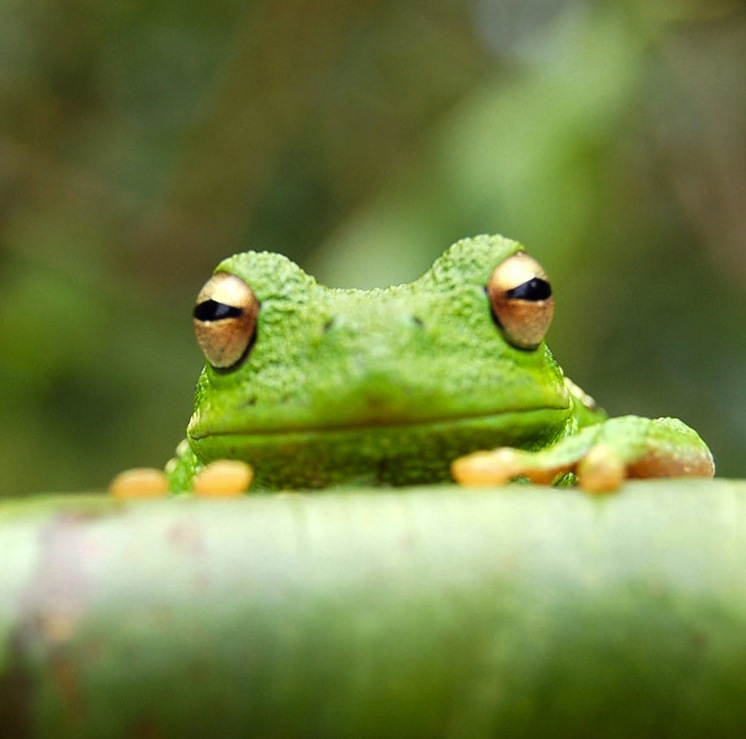
\includegraphics[width=\hsize]{frog}
\caption{A half-columnwidth image using wrapfigure, to be used sparingly. Note that using a wrapfigure before a sectional heading, near other floats or page boundaries is not recommended, as it may cause interesting layout issues. Use the optional argument to wrapfigure to control how many lines of text should be set half-width alongside it.}
\label{fig:halfwidth}
\end{wrapfigure}

Some filler text to sit alongside the half-width figure. \lipsum[1] \lipsum[2]

Really wide figures or tables, that take up the entire page, including the gutter space: use \verb|\begin{fullwidth}...\end{fullwidth}| as in \FIG{fullwidth}. And sometimes you may want to use feature boxes like \BOX{simple}.

\begin{figure}
\begin{fullwidth}
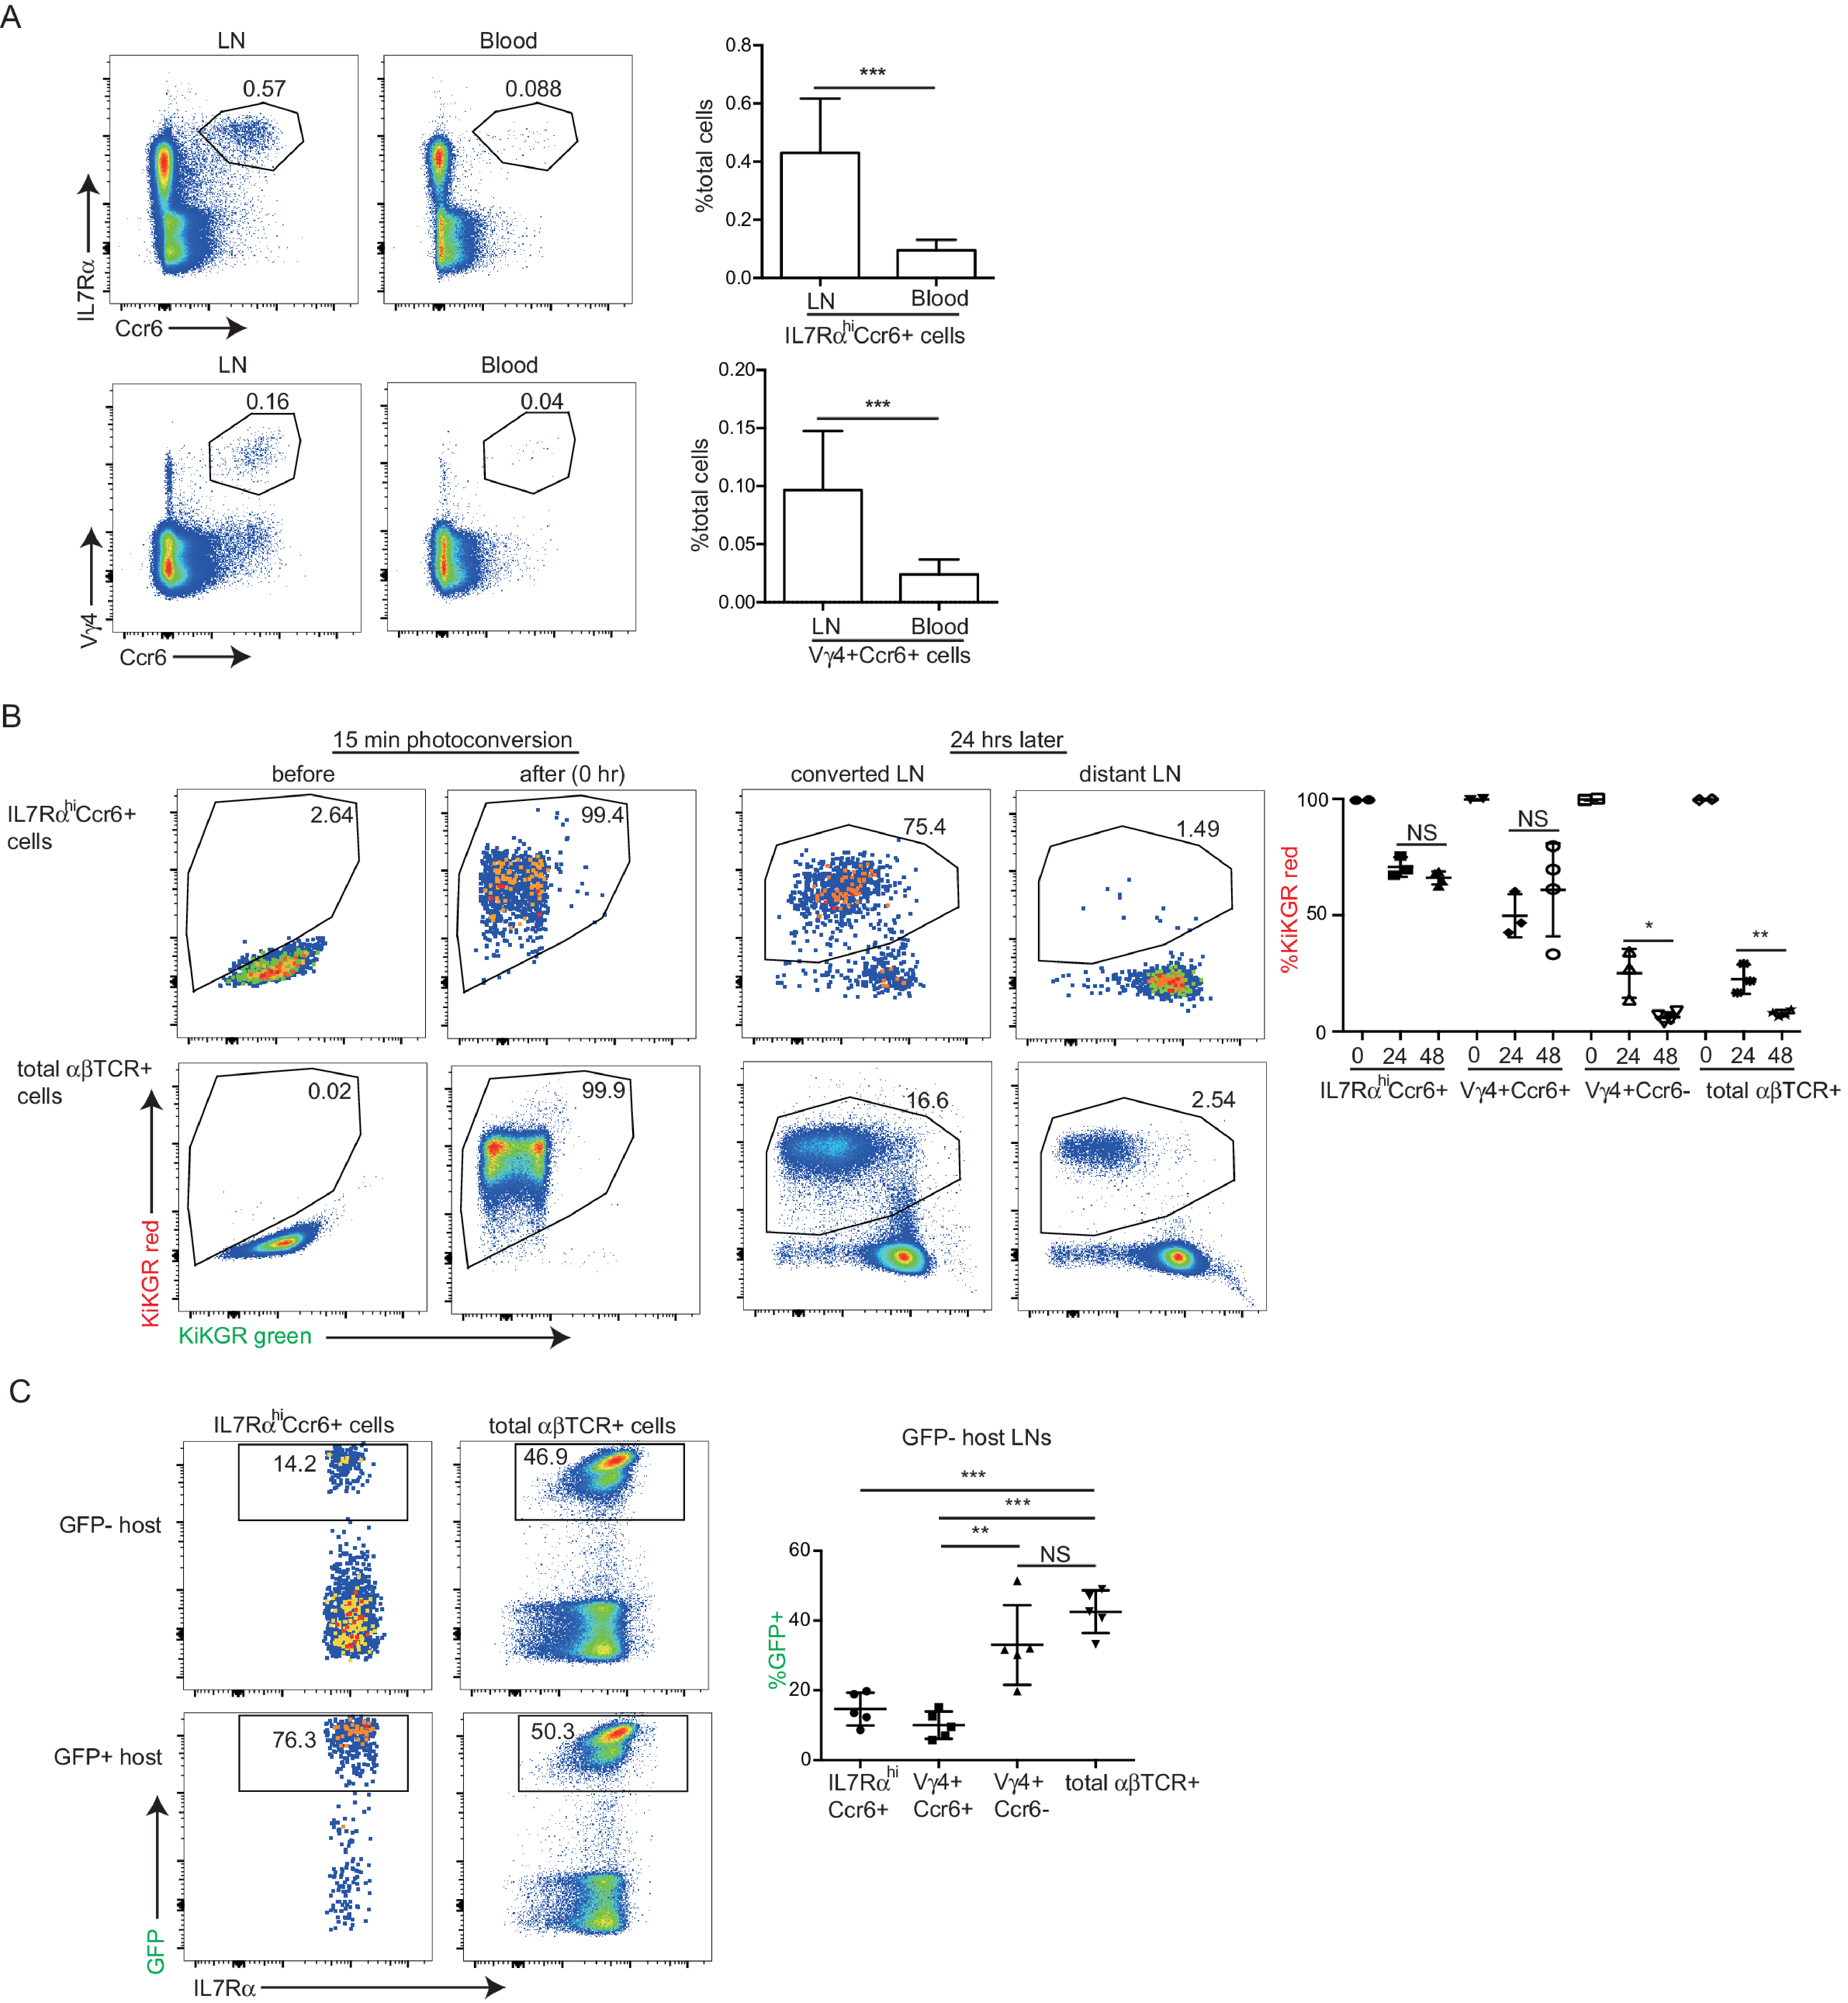
\includegraphics[width=0.95\linewidth]{elife-18156-fig2}
\caption{A very wide figure that takes up the entire page, including the gutter space. A very wide figure that takes up the entire page, including the gutter space. A very wide figure that takes up the entire page, including the gutter space. A very wide figure that takes up the entire page, including the gutter space. A very wide figure that takes up the entire page, including the gutter space. A very wide figure that takes up the entire page, including the gutter space.}
\label{fig:fullwidth}
\figsupp{There is no limit on the number of Figure Supplements for any one primary figure. Each figure supplement should be clearly labelled, Figure 1--Figure Supplement 1, Figure 1--Figure Supplement 2, Figure 2--Figure Supplement 1 and so on, and have a short title (and optional legend). Figure Supplements should be referred to in the legend of the associated primary figure, and should also be listed at the end of the article text file.}{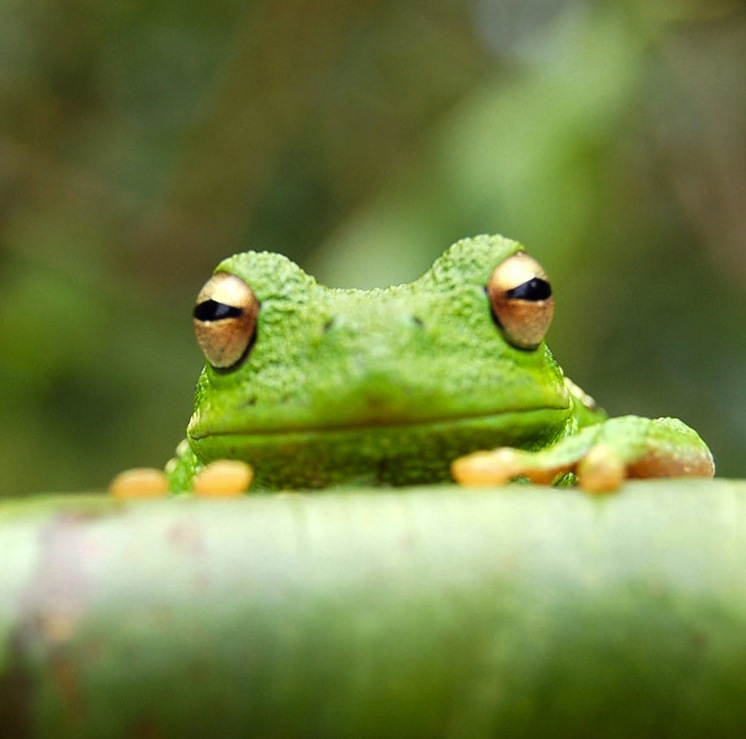
\includegraphics[width=5cm]{frog}}
\end{fullwidth}
\end{figure}

\subsection{Citations}

LaTeX formats citations and references automatically using the bibliography records in your .bib file, which you can edit via the project menu. Use the \verb|\cite| command for an inline citation, like \cite{Aivazian917}, and the \verb|\citep| command for a citation in parentheses \citep{Aivazian917}. The LaTeX template uses a slightly-modified Vancouver bibliography style. If your manuscript is accepted, the eLife production team will re-format the references into the final published form. \emph{It is not necessary to attempt to format the reference list yourself to mirror the final published form.} Please also remember to \textbf{delete the line} \verb|\nocite{*}| in the template just before \verb|\bibliography{...}|; otherwise \emph{all} entries from your .bib file will be listed! 

\begin{featurebox}
\caption{This is an example feature box}
\label{box:simple}
This is a feature box. It floats!
\medskip

\includegraphics[width=5cm]{example-image}
\featurefig{`Figure' and `table' captions in feature boxes should be entered with \texttt{\textbackslash featurefig} and \texttt{\textbackslash featuretable}. They're not really floats.}

\lipsum[1]
\end{featurebox}

\subsection{Mathematics}

\LaTeX{} is great at typesetting mathematics $abc$. Let $X_1, X_2, \ldots, X_n$ be a sequence of independent and identically distributed random variables with $\text{E}[X_i] = \mu$ and $\text{Var}[X_i] = \sigma^2 < \infty$, and let
\begin{equation}
\label{eq:CLT}
S_n = \frac{X_1 + X_2 + \cdots + X_n}{n}
      = \frac{1}{n}\sum_{i}^{n} X_i
\end{equation}
denote their mean. Then as $n$ approaches infinity, the random variables $\sqrt{n}(S_n - \mu)$ converge in distribution to a normal $\mathcal{N}(0, \sigma^2)$.

\lipsum[3] 

\begin{figure}
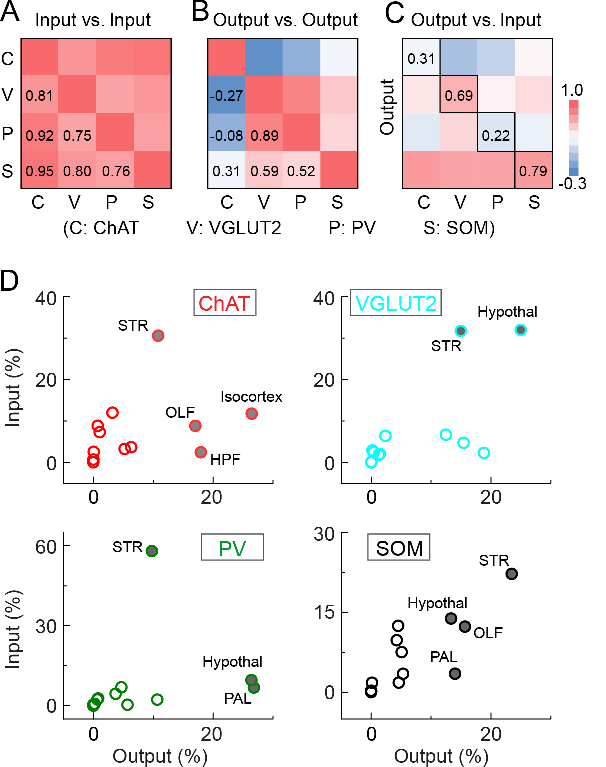
\includegraphics[width=\linewidth]{elife-13214-fig7}
\caption{A text-width example.}
\label{fig:view}
%% If the optional argument in the square brackets is "none", then the caption *will not appear in the main figure at all* and only the full caption will appear under the supplementary figure at the end of the manuscript.
% 
\figsupp[Shorter caption for main text.]
{This is a supplementary figure's full caption, which will be used at the end of the manuscript. 
  \figsuppdata{A data source; see \url{https://doi.org/xxx}}
  \figsuppdata{Another data source.}
  \figsuppsrccode{And the source code.}}
{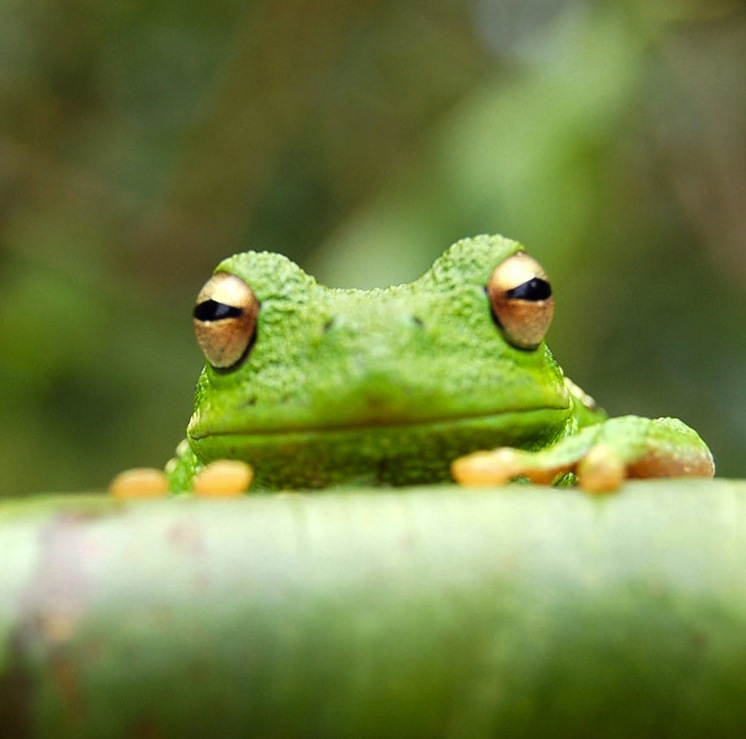
\includegraphics[width=6cm]{frog}}\label{figsupp:sf1}
% 
% 
\figsupp{This is another supplementary figure.}
{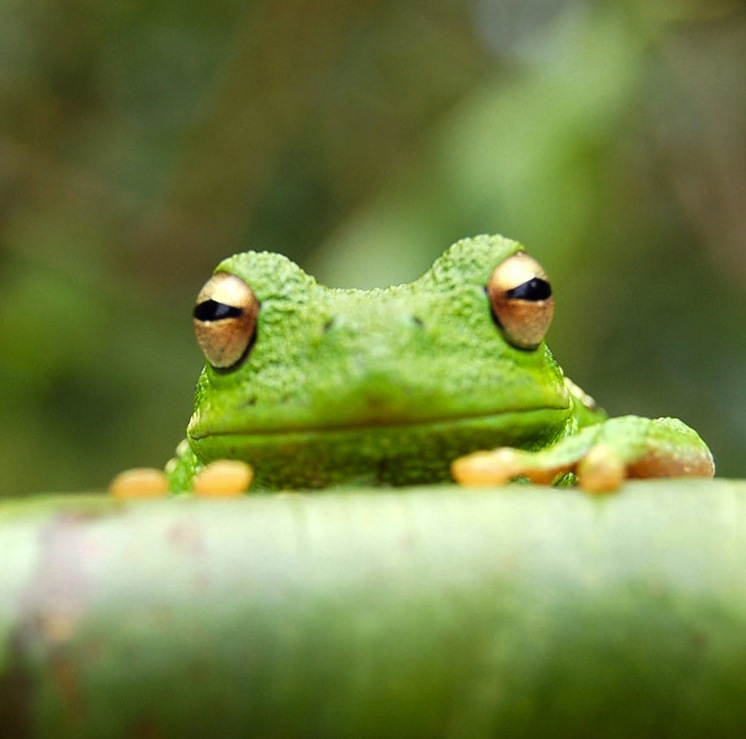
\includegraphics[width=6cm]{frog}}
% 
% 
\videosupp{This is a description of a video supplement.}\label{videosupp:sv1}
\figdata{This is a description of a data source.}\label{figdata:first}
\figdata{This is another description of a data source.}\label{figdata:second}
\figsrccode{This is a description of a source code.}\label{figsrccode:first}
\end{figure}

\subsection{Other Chemistry Niceties}

You can use commands from the \texttt{mhchem} and \texttt{siunitx} packages. For example: \ce{C32H64NO7S}; \SI{5}{\micro\metre}; \SI{30}{\degreeCelsius}; \SI{5e-17}{\Molar}

\subsection{Lists}

You can make lists with automatic numbering \dots

\begin{enumerate}
\item Like this,
\item and like this.
\end{enumerate}
\dots or bullet points \dots
\begin{itemize} 
\item Like this,
\item and like this.
\end{itemize}
\dots or with words and descriptions \dots
\begin{description}
\item[Word] Definition
\item[Concept] Explanation
\item[Idea] Text
\end{description}

Some filler text, because empty templates look really poorly. \lipsum[1]


\section{Acknowledgments}

Additional information can be given in the template, such as to not include funder information in the acknowledgments section.

\nocite{*} % This command displays all refs in the bib file. PLEASE DELETE IT BEFORE YOU SUBMIT YOUR MANUSCRIPT!
\bibliography{elife-sample}

%%%%%%%%%%%%%%%%%%%%%%%%%%%%%%%%%%%%%%%%%%%%%%%%%%%%%%%%%%%%
%%% APPENDICES
%%%%%%%%%%%%%%%%%%%%%%%%%%%%%%%%%%%%%%%%%%%%%%%%%%%%%%%%%%%%

\appendix
\begin{appendixbox}
\label{first:app}
\section{Firstly}
\lipsum[1]

%% Sadly, we can't use floats in the appendix boxes. So they don't "float", but use \captionof{figure}{...} and \captionof{table}{...} to get them properly caption.
\begin{center}
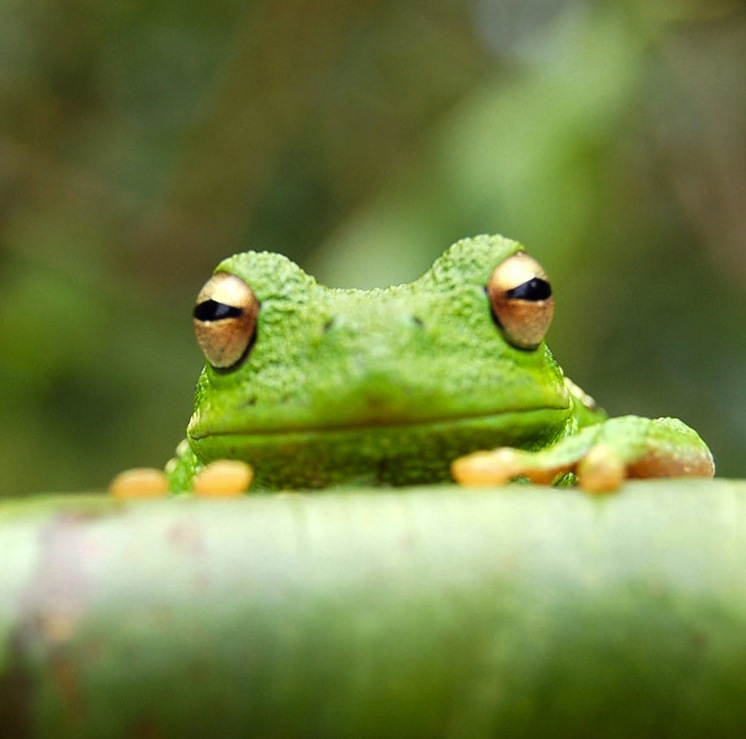
\includegraphics[width=\linewidth,height=7cm]{frog}
\captionof{figure}{This is a figure in the appendix}
\end{center}

\section{Secondly}

\lipsum[5-8]

\begin{center}
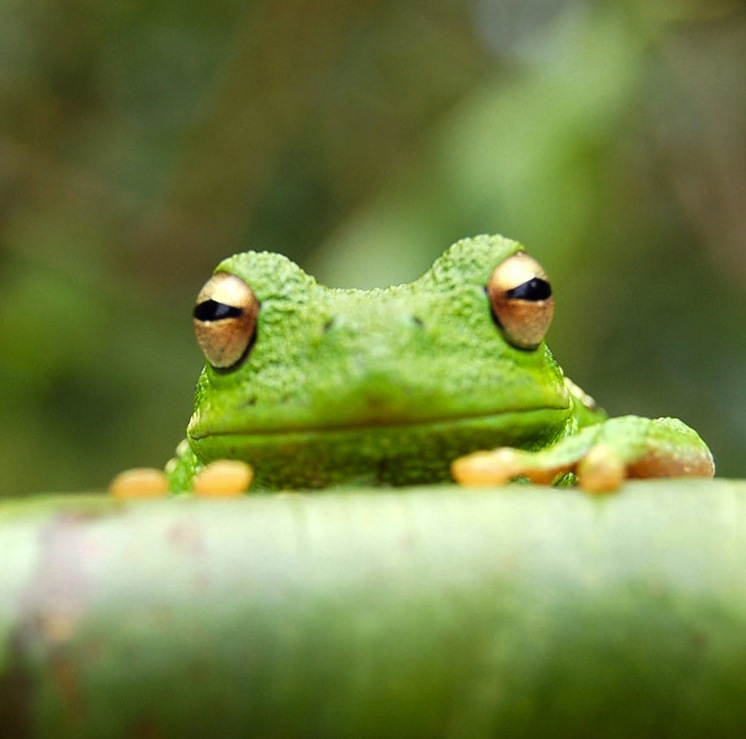
\includegraphics[width=\linewidth,height=7cm]{frog}
\captionof{figure}{This is a figure in the appendix}
\end{center}

\end{appendixbox}

\begin{appendixbox}
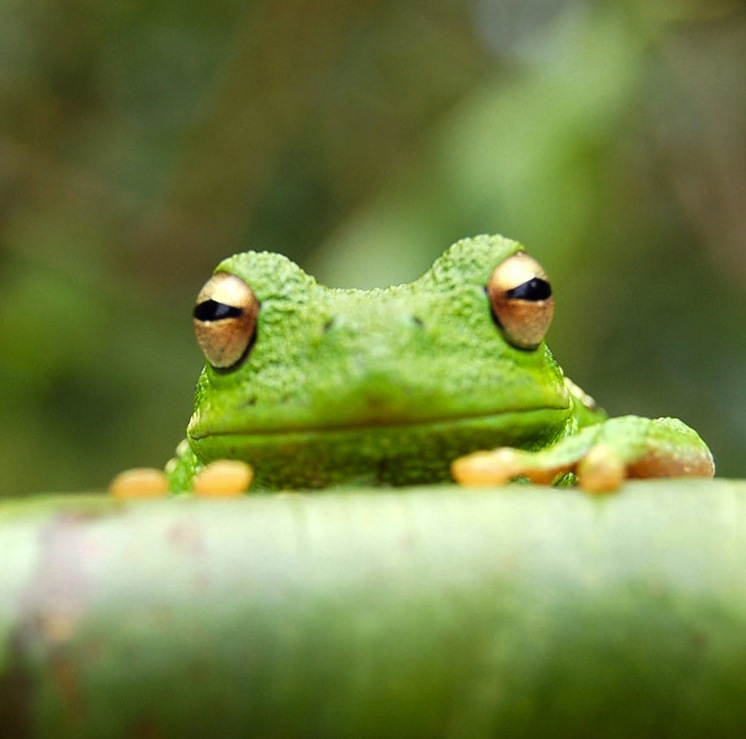
\includegraphics[width=\linewidth,height=7cm]{frog}
\captionof{figure}{This is a figure in the appendix}
\end{appendixbox}
\end{document}
